\documentclass[10pt]{article}
\usepackage[explicit]{titlesec}
\setlength{\parindent}{0pt}
\setlength{\parskip}{1em}
\usepackage{hyphenat}
\usepackage{ragged2e}
\RaggedRight

% These commands change the font. If you do not have Garamond on your computer, you will need to install it.
%\usepackage{garamondx}
\usepackage[T1]{fontenc}
\usepackage{amsmath, amsthm}
\usepackage{graphicx}

% This adjusts the underline to be in keeping with word processors.
\usepackage{soul}
\setul{.6pt}{.4pt}


% The following sets margins to 1 in. on top and bottom and .75 in on left and right, and remove page numbers.
\usepackage{geometry}
\geometry{vmargin={1in,1in}, hmargin={.75in, .75in}}
\usepackage{fancyhdr}
\pagestyle{fancy}
\pagenumbering{gobble}
\renewcommand{\headrulewidth}{0.0pt}
\renewcommand{\footrulewidth}{0.0pt}

% These Commands create the label style for tables, figures and equations.
\usepackage[labelfont={footnotesize,bf} , textfont=footnotesize]{caption}
\captionsetup{labelformat=simple, labelsep=period}
\newcommand\num{\addtocounter{equation}{1}\tag{\theequation}}
\renewcommand{\theequation}{\arabic{equation}}
\makeatletter
\renewcommand\tagform@[1]{\maketag@@@ {\ignorespaces {\footnotesize{\textbf{Equation}}} #1.\unskip \@@italiccorr }}
\makeatother
\setlength{\intextsep}{10pt}
\setlength{\abovecaptionskip}{2pt}
\setlength{\belowcaptionskip}{-10pt}

\renewcommand{\textfraction}{0.10}
\renewcommand{\topfraction}{0.85}
\renewcommand{\bottomfraction}{0.85}
\renewcommand{\floatpagefraction}{0.90}

% These commands set the paragraph and line spacing
\titleformat{\section}
  {\normalfont}{\thesection}{1em}{\MakeUppercase{\textbf{#1}}}
\titlespacing\section{0pt}{0pt}{-10pt}
\titleformat{\subsection}
  {\normalfont}{\thesubsection}{1em}{\textit{#1}}
\titlespacing\subsection{0pt}{0pt}{-8pt}
\renewcommand{\baselinestretch}{1.15}

% This designs the title display style for the maketitle command
\makeatletter
\newcommand\sixteen{\@setfontsize\sixteen{17pt}{6}}
\renewcommand{\maketitle}{\bgroup\setlength{\parindent}{0pt}
\begin{flushleft}
\sixteen\bfseries \@title
\medskip
\end{flushleft}
\textit{\@author}
\egroup}
\makeatother

% This styles the bibliography and citations.
%\usepackage[biblabel]{cite}
\usepackage[sort&compress]{natbib}
\setlength\bibindent{2em}
\makeatletter
\renewcommand\@biblabel[1]{\textbf{#1.}\hfill}
\makeatother
\renewcommand{\citenumfont}[1]{\textbf{#1}}
\bibpunct{}{}{,~}{s}{,}{,}
\setlength{\bibsep}{0pt plus 0.3ex}



%%%%%%%%%%%%%%%%%%%%%%%%%%%%%%%%%%%%%%%%%%%%%%%%%
% Authors: Add additional packages and new commands here.  
% Limit your use of new commands and special formatting.

% Place your title below. Use Title Capitalization.
\title{SIR model with exponentially decaying rate}

% Add author information below. Communicating author is indicated by an asterisk, the affiliation is shown by superscripted lower case letter if several affiliations need to be noted.
\author{Jayanti Prasad}

\pagestyle{empty}
\begin{document}

% Makes the title and author information appear.
\vspace*{.01 in}
\maketitle
\vspace{.12 in}

% Abstracts are required.
\section*{abstract}
What is the simplest model we can fit to the covid-19 data ?
% Keywords are required.
\section*{introduction}

The simplest model of epidemic is given by the Succeptable-Infected-Removed (SIR) model
in which the entire population (of a country) falls in one of the three compartments:
'S', 'I' and 'R'. In the beginning of an epidemic almost all the population falls in 'S'
with few cases in 'I' and none in R'. Once the epidemic progresses a fraction in the 'S'
compartment decreses with rate $\beta$ and increases in 'I' with the same rate. Now some 
fraction of population 'moves' out of the 'I' compartment and goes into the 'R' compartment,
with rate $\gamma$, basically these are the people who eventually die or recover with immunity
so that they never become infected again. The dynamic is 






The section outline below is obligatory for STEM fields. For creative fields, it might be subject specific; however, \textit{References}, \textit{About Student Author(s)}, and \textit{Press Summary} sections are required. 

In-text reference citations should support statements made on behalf of others.\cite{journal} See detailed comments about references on the next page. 

\ul{To underline a portion of text}, use the \verb+\ul{}+ command in lieu of \verb+\underline{}+

For units, check for space between a number and its unit (exceptions are percent \% and degree $^\circ$ signs). Use Symbol font for micro ($\mu$), not u or $u$. Latin words (\textit{etc., et al., i.e.}), and Latin names of species, (e.g. \textit{E. coli}) and web sites should be italicized in text and in references. In a sentence, spell out numbers under $10$ instead of using a number (\textit{i.e.}, use six and not $6$).

When you need to refer to \textbf{Figure \ref{sample image}}, \textbf{Table \ref{sample table}}, \textbf{Scheme 1}, \textbf{Step 1}, and \textbf{Equation \ref{equ1}} please bold those words in the text and in the title. The table itself should be centered.

\begin{table}[htp!]
\begin{center}
\begin{tabular}{ | c | c | c | c | }
\hline
 & \textbf{Column 1} & \textbf{Column 2} & \textbf{Column 3} \\ 
 \hline
 \textbf{Row 1} & a & b & c \\  
 \hline
\end{tabular}
\caption{The table itself should be centered. The title should be aligned to left or centered, whichever looks better. The table title In AJUR goes below the table and ends with a period. Please bold column and row titles.}
\label{sample table}
\end{center}
\end{table}

\section*{methods and procedures}

\subsection*{Subsections' titles should be mixed case and italicized.}
Use sections and subsections without numbers, by using \verb+\section*{}+ and \verb+\subsection*{}+ with an \verb+*+. Describe technical details of your work,\cite{journal,chapters} mention the IRB/IACUC permissions' numbers when working with humans/animals.

\section*{results}
\subsection*{Subsections' titles should be mixed case and italicized.}
When referring to other sections (such as \textit{Introduction}), italicize them. Figures should not be wrapped- regular text goes above and below them. Figures should be centered.

%You will be uploading any pictures to the files on the left.
\begin{figure}[ht!]
\centering
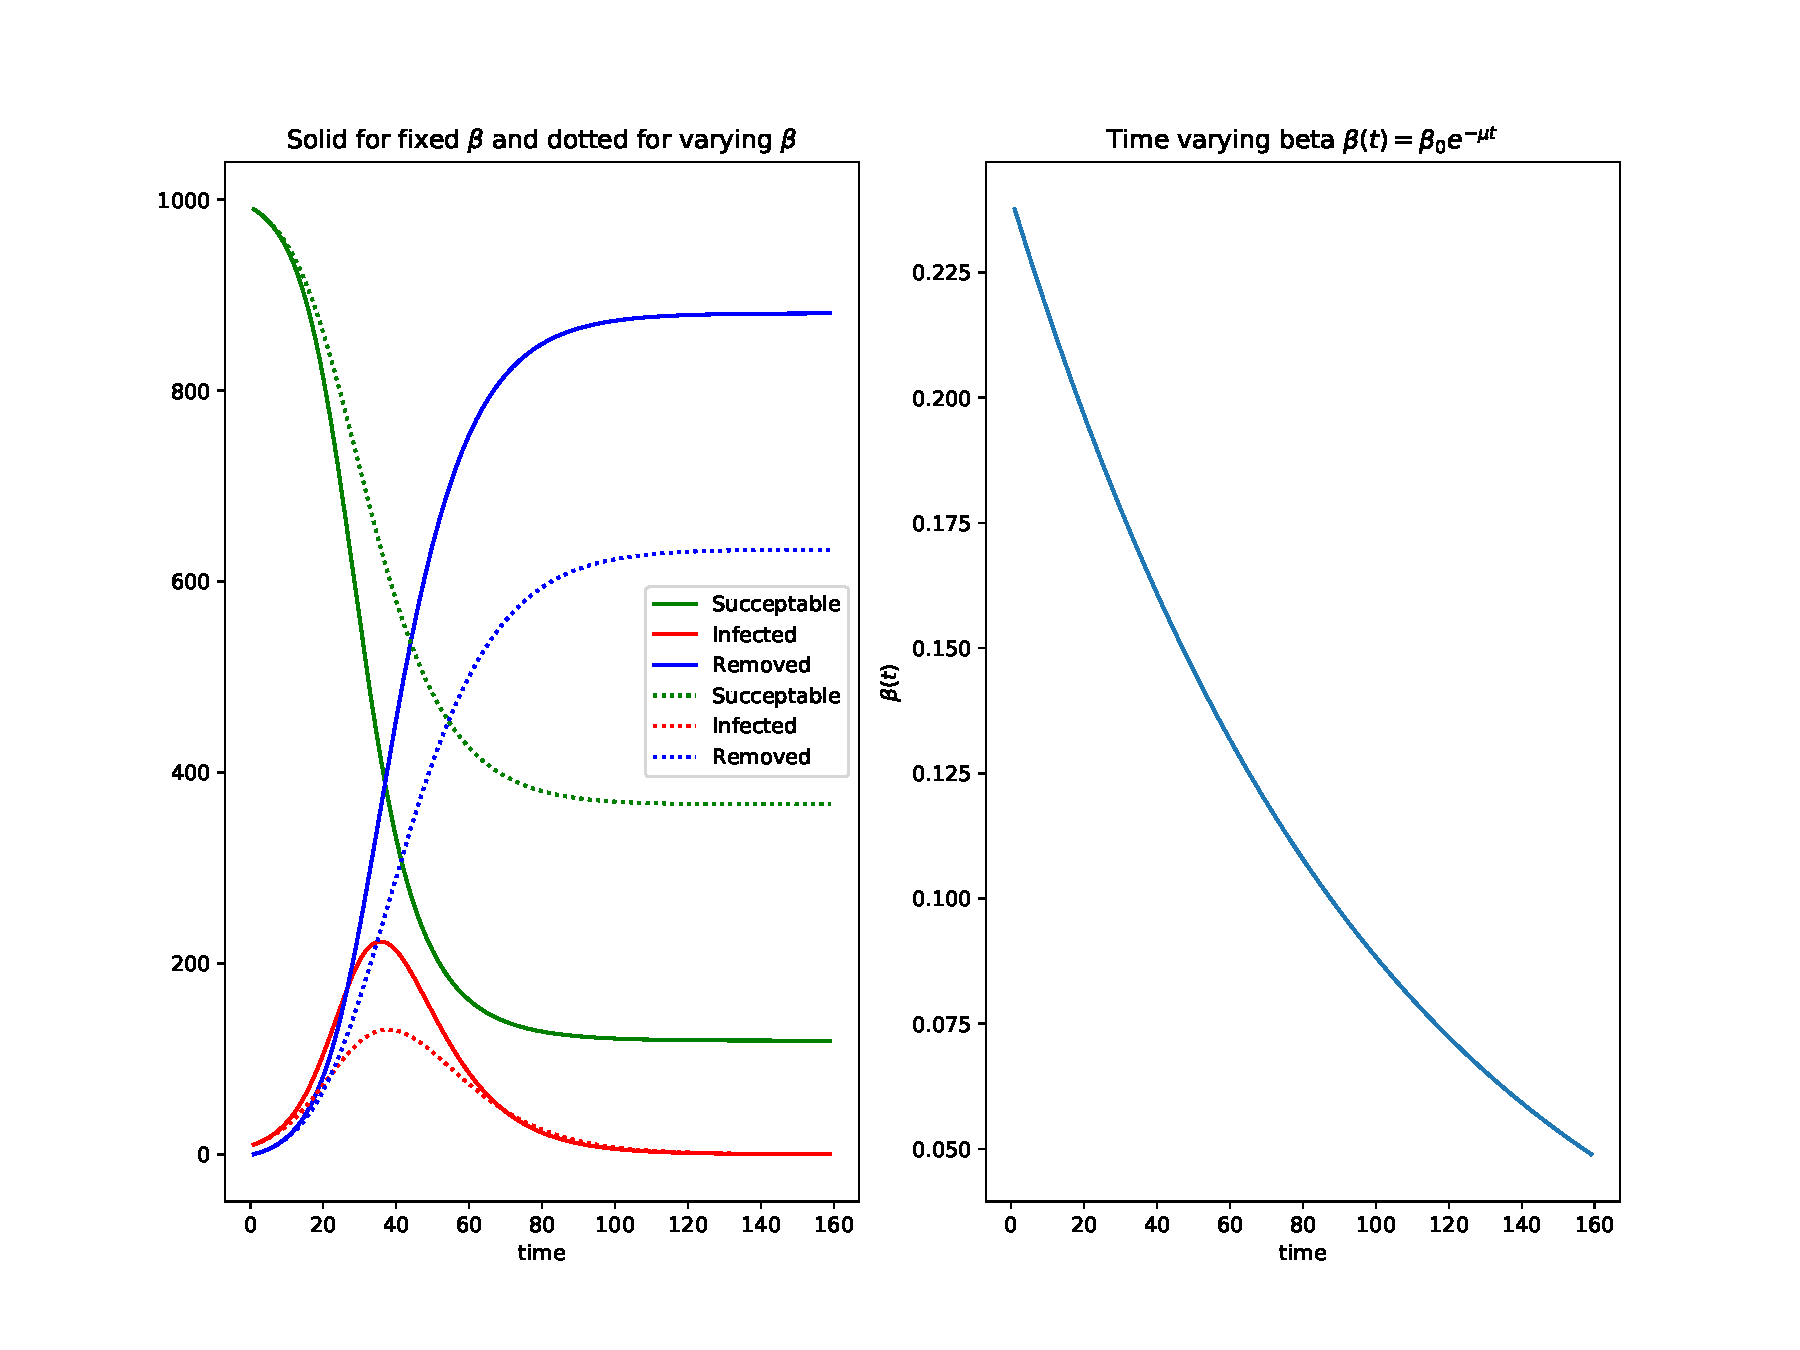
\includegraphics[width=0.5\textwidth]{sir_with_varing_beta.pdf}
\caption{Figure and scheme titles go below figures. Title may be left-aligned or centered, whichever looks better. It may be the width of the page or the width of the figure. There is no space between the figure and the figure title. Figure title ends with a period.}\label{sample image}
\end{figure}

\section*{discussion}
Use tables and figures as described above. Use proper referencing.\cite{web}

All reaction schemes and mathematical equations, unless used in-line, must be centered and not wrapped. The associated scheme or equation number should be bolded, on the right hand side of the page with a period after it. When referring to  in text, do not period after the scheme number.

\begin{equation}
x= \dfrac{-b \pm \sqrt{b^2 - 4ac}}{2a} \label{equ1}
\end{equation}

This is the appropriate way to display an equation.

\begin{verbatim}
\begin{equation} 
x= \dfrac{-b \pm \sqrt{b^2 - 4ac}}{2a} \label{equ1}
\end{equation}
\end{verbatim}

 Using the \$\$ method, the \verb+ \[, \] + environment, and the \verb+equation*+ environment produce unnumbered equations and should be avoided. 

In multiline equations, label only the last line.

\begin{align*}
x &= \dfrac{-b \pm \sqrt{b^2 - 4ac}}{2a} \\
  &= 2 \pm 3i \num \label{eqn2}
\end{align*}

This template automatically loads usual \verb+amsthm+ and \verb+amsmath+ packages.  Additional packages should be loaded in the preamble.  

\section*{conclusions}
Describe major outcomes, novelty, and significance of your work. Future work may be noted.

\section*{acknowledgements}
This section is optional. The authors thank and not ``would like to thank'' such and such an organization or person. Co-authors should not be listed here.
%Note correct LaTeX quotations above. Do not use the " symbol, but rather double ` followed by double '

%There will be no "notes on references" section in your final draft, please remove this section heading.
\section*{notes on references}

Use no indents. Follow the style given in the examples (journals and serial publications;\cite{journal} chapters and monographs;\cite{chapters} web sources,\cite{web} correspondingly) below. All references in text must be in order of appearance. Please include all authors, the complete title, and inclusive pagination, \textit{e.g.}, 1234--1237, not 1234--7; \ul{please make sure to use en-dash} (in \LaTeX, use \verb+--+) \ul{and not the regular dash or em-dash to indicate duration between page numbers or years.} The publication year should follow authors in parentheses. Supply DOI numbers whenever possible. \textit{Book titles} and \textit{web sites} are italicized. \textit{Titles of journals} should be abbreviated according to http://www.abbreviations.com/jas.php. \textbf{\ul{Reference accuracy is critical. It is authors responsibility to carefully check each reference.}} 

In the text, separate superscripted numbers by comma and space,\cite{journal,chapters} they should be separated by an en-dash if the consecutive list of more than two numbers is used.\cite{journal,chapters,web} List them AFTER punctuation (be it comma or period) with no space.

\begin{thebibliography}{9} %If you have more than 9 sources listed, replace this "9" with "99".

\bibitem{journal} Marquez, V., Frohlich, T., Armache, J. P., Sohmen, D., Donhofer, A., Mikolajka, A., Berninghausen, O., Thomm, M., Beckmann, R., Arnold, G. J., and Wilson, D. N. (2011) Proteomic characterization of archaeal ribosomes reveals the presence of novel archaeal-specific ribosomal proteins, \textit{J Mol Biol} 405, 1215--1232. \textit {https://doi.org/10.33697/ajur.2019.003}


\bibitem{chapters} Fierke, C. A., and Hammes, G. G. (1996) Transient Kinetic Approaches to Enzyme Mechanisms, in \textit{Contemporary Enzyme Kinetics and Mechanism} (Purich, D., Ed.) 2nd ed., 1--35, Academic Press, New York.

\bibitem{web} Agricultural Research Service, U.S.D.A. National Nutrient Database for Standard Reference, Release 26, \textit{http://ndb.nal.usda.gov/ndb/search/list} (accessed Mar 2014)
\end{thebibliography}

% The About the Student Author section is NOT optional.  Write a paragraph about the student; see previous journal editions for examples.
% If there is more than one student author, you must move the comment below.
\section*{about the student author}
%\section*{about the student authors}
John Smith and Jane Smith will graduate in \ldots, \textit{etc.}

% The Press Summary section is NOT optional.  Write a paragraph describing the paper in a manner suitable for the press; see previous journal editions for examples.
\section*{press summary}

Please rewrite your abstract so that it captures in few sentences the scope and focus of your publication but could be easily understood by the general public and hopefully shows why your work is exciting and important.

Once done, review these guidelines and the entire document. Make sure that images are exactly where you want them, not at the end of the text. Insert page brakes to avoid orphan titles, words, or sentences being separated out at the end or the top of a page. If any questions remain, please e-mail editor@ajuronline.org.

When you are ready to submit your article, use the share button above and send the read and edit  link.
\end{document}
